\scanpage{34}

2. \uline{Accouplements définis par une biextension}.

2.1. Soit $n$ un entier $>0$, et supposons qu'on a
\[
(2.1\deleted{)}.1)\qquad nP=P.
\]
\noindent\makebox[0pt][l]{\begin{tikzpicture}[overlay,x=1em,y=1ex]
\draw (-2.7,-.40)..controls(-2.77,-.58)and(-2.75,-.69)..(-2.55,-.65)
..controls(-1.1,-.48)and(.15,-.55)..(.65,-.50);
\draw (-2.3,-1.05)..controls(-.8,-.91)and(.7,-.96)..(1.2,-.93);
\draw (1.7,-.94)..controls(1.9,-.91)and(2.1,-.96)..(2.05,-1.13);
\end{tikzpicture}}Considérons alors l'homomorphisme composé

(2.1.2)
\diagram{\begin{tikzcd}[ampersand replacement=\&,column sep=large]
\operatorname{Biext}^{\inserted{1}}(P,Q;G)
\arrow[r]\arrow[rr,bend left=20,"\varphi^n"]
\&\operatorname{Biext}^{\inserted{1}}(P,{}_nQ;G)\arrow[r,"\sim"]
\&\operatorname{Hom}({}_nP\otimes{}_nQ;G)
\end{tikzcd}},

où la première flèche est la restriction à $(P,{}_nQ)$, et la deuxième est l'isomorphisme (1.3.\deleted{5}6). Il permet, à tout élément
\makebox[0pt][l]{\begin{tikzpicture}[overlay,x=1em,y=1ex]
\draw (.10,1.2)..controls(1.2,2.05)and(9.7,2.05)..(11.55,1.15)
..controls(12.2,.5)and(12.1,-.8)..(10.9,-1.1)
..controls(6.2,-1.55)and(.7,-1.2)..(-.38,-.25)
..controls(-.52,.12)and(-.48,.66)..(-.35,.9);
\draw (-.15,1.15)..controls(2,2.25)and(10.5,2.0)..(11.8,.85)
..controls(12.45,-.1)and(11.65,-1.2)..(9.8,-1.35)
..controls(5.7,-1.55)and(.6,-1.32)..(-.35,-.55);
\draw[->](-.35,-.55)..controls(-2.9,-1.9)and(-7.8,-.95)..(-10.0,-2.25);
\end{tikzpicture}}$\xi\in\operatorname{Biext}(P,Q;G)$,

(2.1.3)

à fortiori à toute biextension
\makebox[0pt][l]{\begin{tikzpicture}[overlay,x=1em,y=1ex]
\draw (.03,2.3)..controls(-.4,3.8)and(1.0,4.0)..(1.02,2.95);
\draw (1.04,2.65)..controls(1.05,2.0)and(.57,1.7)..(.40,.6);
\draw (.40,.6)..controls(.20,1.7)and(.03,1.9)..(.03,2.3);
\end{tikzpicture}}\raisebox{1.7ex}{\inserted{$E$}}
de $(P,Q)$ par $G$, de faire correspondre un\deleted{e \unsure{forme homomorphisme}} accouplement bilinéaire
\reversemarginpar
\margin{\makebox[0pt][l]{
\begin{tikzpicture}[overlay,x=1em,y=1ex]
\draw (.72,1.75)..controls(-.7,2.35)and(-1.2,-1.3)..(-.15,-2.0)
..controls(1.35,-2.35)and(1.65,.75)..(1.02,1.45);
\end{tikzpicture}}$\varphi$}
\normalmarginpar
\[
(2.1.4)\qquad
\phi_{\inserted{\xi}}\text{ ou }\phi^n_{\inserted{\xi}}:{}_nP\times{}_nQ\longrightarrow G,
\]
qu'on appelle l'accouplement \uline{associé à} $\xi$ (ou à la biextension $E$).

2.2. Soit $\deleted{\unsure{ni|n'}}$ $n'$ un multiple de $n$,
\[
n'=mn,
\]
et supposons qu'on ait la relation (plus forte que (2.1.1))
\[
(2.2.1)\qquad n'P=P\quad\text{i.e.}\quad mnP=P,
\]
d'où comme en (2.1.4), pour toute $\xi\in\operatorname{Biext}(P,Q;G)$, un\deleted{e} accouplement
\[
\phi^{n'}_{\inserted{\xi}}:{}_{n'}P\times{}_{n'}Q\longrightarrow G.
\]
\deleted{Les relations entre cet accouplement et}\inserted{Il est lié à} l'accouplement $\phi^n_{\inserted{\xi}}$ \deleted{est donné} par la commutativité du diagramme suivant (\deleted{qu'on laisse au lecteur le soin d'établir).}\inserted{cf. 2.3 ci-dessous pour une démonstration):}

(2.2.2)
\diagram{\begin{tikzcd}[ampersand replacement=\&,column sep=small,row sep=large]
{}_{n'}P\arrow[d,"m"']
\&\times
\&{}_{n'\deleted{\unsure{n}}}Q\deleted{\unsure{Q}}\arrow[d,"m"]\arrow[rr,"\phi^{n'}_{\inserted{\xi}}"]
\&\&{}_{n'}G\arrow[d,"m"]\\
\deleted{\unsure{P|Q}}{}_nP
\&\deleted{\times}\times
\&{}_nQ\arrow[rr,"\phi^n_{\inserted{\xi}}"]
\&\&{}_nG
\end{tikzcd}},
\noindent\makebox[\linewidth][l]{\small
\makebox[0pt][l]{\begin{tikzpicture}[overlay,x=\linewidth,y=1ex]
\draw (-.01,-2.0)..controls(-.02,-.2)and(.025,.1)..(.12,-.35)
..controls(.38,-.70)and(.78,-.52)..(.96,-.45)
..controls(1.055,-.35)and(1.06,2.5)..(.98,2.6)
..controls(.94,2.5)and(.89,2.35)..(.85,2.2);
\end{tikzpicture}}
\inserted{où les flèches verticales sont induites par la multiplication par $m=n'/n$.}}

Notons maintenant que moyennant (2.1.1), on peut prendre pour $n'$ n'importe quelle puissance de $n$. En particulier, soit
\makebox[0pt][l]{\begin{tikzpicture}[overlay,x=1em,y=1ex]
\draw (.55,2.7)..controls(-.15,3.7)and(-.8,-1.8)..(-.45,-2.4)
..controls(.20,-3.0)and(1.2,-1.7)..(1.03,1.9);
\end{tikzpicture}}$\ell$
un nombre premier, et supposons que\deleted{\illegible{1}} l'on ait
\reversemarginpar
\margin{\makebox[0pt][l]{
\begin{tikzpicture}[overlay,x=1em,y=1ex]
\draw (.75,2.1)..controls(.35,3.1)and(-.85,.4)..(-.55,-1.75)
..controls(-.35,-3.3)and(1.4,-2.2)..(1.6,.5)
..controls(1.7,1.4)and(1.45,2.1)..(1.10,2.35);
\end{tikzpicture}}$\ell$}
\normalmarginpar
\[
(2.2.3)\qquad
\makebox[0pt][l]{
\begin{tikzpicture}[overlay,x=1em,y=1ex]
\draw (.55,2.5)..controls(-.25,2.9)and(-1.0,-1.7)..(-.65,-2.35)
..controls(.0,-2.65)and(1.0,.4)..(.82,1.8);
\end{tikzpicture}}\ell P=P,
\]
et considérons le système des accouplements
\margin{33}
